\chapter{Introduzione}

Il corso mirà allo sviluppo di applicazioni di grande portata. Questo implica l'insegnamento della programmazione a eventi, alle interfacce grafiche (SWING e JAVAFX/FXML), la programmazione parallela (processi e thread) e la programmazione in rete (socket).

\section{La progettazione a oggetti}

\dfn{Oggetti}{Bisogna capire i tipi di \textbf{entità} da rappresentare, le azioni e il modo in cui interagiscono e comunicano. Il mondo è costituito da oggetti. }

\ex{Simulatore di guida}{
In un simulatore di guida bisogna:

\begin{itemize}
    \item modellare i semafori (per regolare il traffico);
    \item modellare le macchine (accese, spente, in movimento);
    \item modellare la strada (passiva);
    \item non si modellano i cani che attraversano la strada.
\end{itemize}
}

\nt{Bisogna modellare solo le entità ritenute interessanti.}

\dfn{Stato e comportamento}{Ogni oggetto ha uno \textbf{stato} (che è costituito da i suoi attributi) e un \textbf{comportamento} (che è modellato come un insieme di metodi). Il comportamento va a modificare lo stato degli oggetti.}
\pagebreak
\begin{figure}[h]
\caption{Esempio di progettazione a oggetti}
\begin{center}
    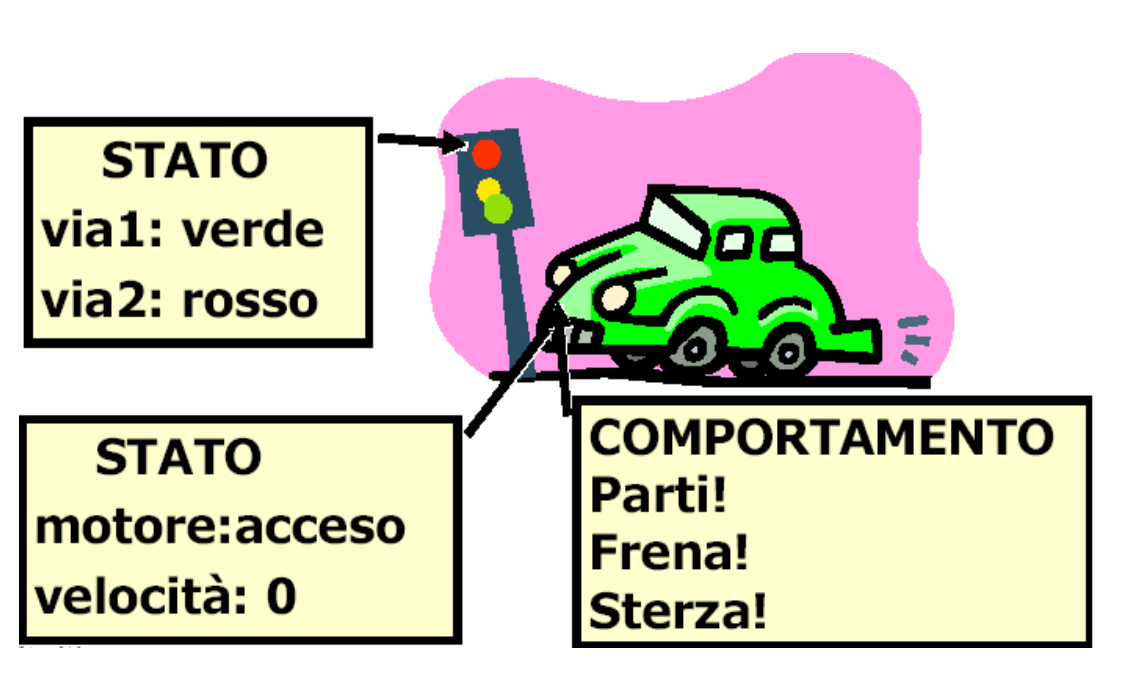
\includegraphics[scale=0.3]{images/intro/Guida.png}
\end{center}
\end{figure}

\subsection{Oggetti e realtà}

Ogni individuo ha una visione limitata della realtà con una propria identità, uno stato e un comportamento diverso. 

\dfn{Incapsulamento}{Gli stati si basano sul principio dell'\textbf{incapsulamento}: uno stato "appartiene" a un oggetto, per cui un utente esterno non può manipolarlo.}

\dfn{Delega}{I comportamenti si basano sul principio della \textbf{delega}: chi fa la richiesta non vuole conoscere in dettaglio come sia eseguita.}

\dfn{Un programma}{Un programma viene visto come un insieme di oggetti che comunicano l'un l'altro invocando metodi. Un oggetto può contenere riferimenti ad altri oggetti. Ogni oggetto ha un tipo (\textbf{classe}). 

Una struttura dati è vista come un insieme di operazioni. Per esempio, una \textbf{lista} (astratta) è una sequenza ordinata di dati che possono essere letti sequenzialmente e in cui si può inserire/rimuovere un dato in una posizione i.}

\cor{\textbf{Object-oriented design.}}{La progettazione orientata agli oggetti. Si mettono insieme sistemi software visti come collezioni di oggetti.}

\subsection{Programmazione procedurale vs. Programmazione object-oriented}

In questa sezione è presente un breve confronto.

\dfn{Programmazione procedurale}{La \textbf{programmazione procedurale} si concentra sull'organizzare le procedure che operano sui dati. Il suo paradigma è: eseguire una sequenza di passi per raggiungere il risultato. }

\nt{Il programma viene visto come:  ALGORITMI + STRUTTURE DATI}

\dfn{Programmazione object-oriented (O-O)}{La \textbf{programmazione object-oriented} si concentra sulle entità incapsulando dati e operazioni. Il suo paradigma è legato a responsabilità e deleghe.}

\nt{Il programma viene visto come:   OGGETTI (DATI + ALGORITMI) + COLLABORAZIONE (INTERFACCE)}

\section{Sviluppare a oggetti}

Si vedono gli oggetti come fornitori di servizi. Ogni oggetto svolge un piccolo servizio, ma tutti insieme forniscono un grande servizio.

\subsection{Come si fa?}

Si vanno a vedere i sostantivi/nomi che vengono utilizzati perchè diventeranno classi. I verbi andranno a indicare le azioni e i metodi.

\dfn{Classi e istanze}{Una \textbf{classe} è un'idea astratta che rappresenta caratteristiche comuni a tutte le istanze di un oggetto. Un'\textbf{istanza} è un singolo oggetto "concreto".

Un'istanza ha:

\begin{itemize}
    \item un'identità;
    \item uno stato;
    \item un comportamento.
\end{itemize}
}

\nt{Dobbiamo chiederci:

\begin{itemize}
    \item quali sono le entità fondamentali da modellare e quali sono i dati di cui abbiamo bisogno?;
    \item di quante istanze, per ogni concetto, abbiamo bisogno?.
\end{itemize}
}

\dfn{Interfacce e implementazioni}{
L'\textbf{interfaccia} è la \textit{firma} dei metodi, ossia la "vista esterna". L'\textbf{implementazione} è la "vista interna", come è fatto un metodo.
}

\nt{Oltre ancora bisogna capire, di volta in volta, quale tipo di servizio va offerto e mostrato al mondo. Alcuni dati vanno bene pubblici, altri devono essere privati.}

\dfn{Modularità}{Un'altra componente è la \textbf{modularità} cioè la suddivisione in una serie di componenti indipendenti.
}

\dfn{Gerarchie}{Infine si hanno le gerarchie:

\begin{itemize}
    \item part-of hierarchy: gerarchia di parti;
    \item kind-of hierarchy: gerarchia di classi e sotto-classi.
\end{itemize}
}

\ex{Vantaggi di un approccio O-O}{

\begin{itemize}
    \item [\textcolor{green}{\usym{1F5F8}}] Riuso e maggiore leggibilità;
    \item [\textcolor{green}{\usym{1F5F8}}] Dimensioni ridotte;
    \item [\textcolor{green}{\usym{1F5F8}}] Compatibilità e portabilità;
    \item [\textcolor{green}{\usym{1F5F8}}] Estensione e modifica più semplici;
    \item [\textcolor{green}{\usym{1F5F8}}] Manutenzione del software semplificata;
    \item [\textcolor{green}{\usym{1F5F8}}] Migliore gestione del team di lavoro.
\end{itemize}
}

\nt{Nella programmazione O-O occorre conoscere l'interfaccia di una classe, ma non necessariamente la sua implementazione.}






